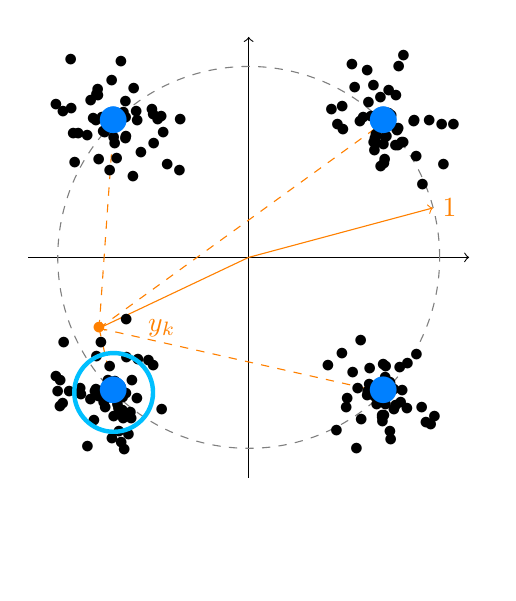
\begin{tikzpicture}
    \draw[->] (-2.8,0) --++ (5.6,0) node[right]{$\calI$};
    \draw[->] (0,-2.8) --++ (0,5.6) node[right]{$\calQ$};
    \draw[dashed, color = gray] (0,0) circle (2.425);
    \draw[orange,->] (0,0) --++ (2.34,0.628) node[right]{$1$};
    \draw[orange,->] (0,0) --++ (-1.9,-0.9) node[right = 5mm]{$y_k$};

    \node[color = blue!50!cyan] at (1.715,1.715) (a){\Huge $\bullet$};
    \node[color = blue!50!cyan] at (1.715,-1.715) (b){\Huge $\bullet$};
    \node[color = blue!50!cyan] at (-1.715,1.715) (c){\Huge $\bullet$};
    \node[color = blue!50!cyan] at (-1.715,-1.715) (d){\Huge $\bullet$};
    \node[color = orange] at (-1.9,-0.9) (e){$\bullet$};

    \draw[color = orange,dashed] (e.center) -- (a.center);
    \draw[color = orange,dashed] (e.center) -- (b.center);
    \draw[color = orange,dashed] (e.center) -- (c.center);
    \draw[color = orange,dashed] (e.center) -- (d.center);

    \foreach \x in {1.70,1.705,1.71,1.715,1.72,1.725,1.73}
        {\foreach \y in {1.70,1.705,1.71,1.715,1.72,1.725,1.73}
            {\draw (\x+rand*rand,\y+rand*rand) node{$\bullet$};}
        }

    \foreach \x in {-1.70,-1.705,-1.71,-1.715,-1.72,-1.725,-1.73}
        {\foreach \y in {1.70,1.705,1.71,1.715,1.72,1.725,1.73}
            {\draw (\x+rand*rand,\y+rand*rand) node{$\bullet$};}
        }

    \foreach \x in {1.70,1.705,1.71,1.715,1.72,1.725,1.73}
        {\foreach \y in {-1.70,-1.705,-1.71,-1.715,-1.72,-1.725,-1.73}
            {\draw (\x+rand*rand,\y+rand*rand) node{$\bullet$};}
        }

    \foreach \x in {-1.70,-1.705,-1.71,-1.715,-1.72,-1.725,-1.73}
        {\foreach \y in {-1.70,-1.705,-1.71,-1.715,-1.72,-1.725,-1.73}
            {\draw (\x+rand*rand,\y+rand*rand) node{$\bullet$};}
        }

    \node[color = blue!50!cyan] at (1.715,1.715) (a2){\Huge $\bullet$};
    \node[color = blue!50!cyan] at (1.715,-1.715) (b2){\Huge $\bullet$};
    \node[color = blue!50!cyan] at (-1.715,1.715) (c2){\Huge $\bullet$};
    \node[color = blue!50!cyan] at (-1.715,-1.715) (d2){\Huge $\bullet$};

    \draw[color = blue!50!cyan!50!cyan, ultra thick] (-1.715,-1.715) circle (0.5);

    \draw[white] (0,-4) --++ (0,0.5);
\end{tikzpicture}
